\documentclass[10pt]{article}
\usepackage[ngerman]{babel}
\usepackage[utf8]{inputenc}
\usepackage[T1]{fontenc}
\usepackage{amsmath}
\usepackage{amsfonts}
\usepackage{amssymb}
\usepackage[version=4]{mhchem}
\usepackage{stmaryrd}
\usepackage{bbold}
\usepackage{graphicx}
\usepackage[export]{adjustbox}
\graphicspath{ {./images/} }

\title{Hauptprüfung Abiturprüfung 2024 - Leistungsfach }

\author{Alexander Schwarz\\
www.mathe-aufgaben.com}
\date{}


\begin{document}
\maketitle
 Baden-Württemberg

\section*{Aufgabe I 1.1}
Gegeben ist die Schar der in $\mathbb{R}$ definierten Funktionen $f_{a ; b}(x)=a x^{3}-b x$ mit $a, b \in \mathbb{R}^{+}$. Die Abbildung zeigt den Graphen einer der Funktionen der Schar.\\
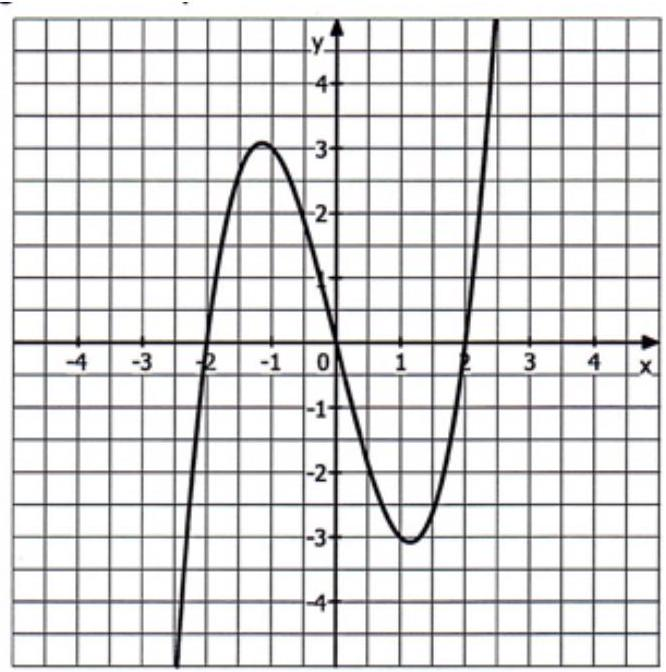
\includegraphics[max width=\textwidth, center]{2025_04_24_115a845b97d0fe4b6479g-2}\\
a) Begründen Sie, dass jeder Graph der Schar symmetrisch bezüglich des Koordinatenursprungs ist.\\
b) Weisen Sie in Abhängigkeit von $a$ und $b$ nach, dass der Graph von $f_{a ; b}$ einen Tiefpunkt mit der x-Koordinate $\sqrt{\frac{b}{3 a}}$ hat. Begründen Sie, dass er zudem einen Hochpunkt besitzt und dass dieser eine kleinere $x$-Koordinate hat als der Tiefpunkt.\\
(6 BE)\\
c) Es gibt eine Funktion der Schar, die bei $x=3$ eine Nullstelle hat und deren Graph im vierten Quadranten mit der x-Achse ein Flächenstück mit dem Inhalt 40,5 einschließt. Bestimmen Sie die zugehörigen Werte von a und b.\\
(7 BE)\\
Die Funktion der Schar, deren Graph in der Abbildung dargestellt ist, wird mit f bezeichnet; ihr Funktionsterm ist $f(x)=x^{3}-4 x$.\\
d) Die Tangente an den Graphen von fim Punkt A(2|0), die x-Achse und die Gerade $g$ mit der Gleichung $y=-x-2$ schließen ein Dreieck ein. Berechnen Sie seinen Flächeninhalt.\\
e) Begründen Sie, dass die folgende Aussage richtig ist:

Ist $P$ ein beliebiger Punkt auf dem Graphen von f, so liegt der Mittelpunkt der Verbindungsstrecke von $P$ und dem Koordinatenursprung auf dem Graphen der in $\mathbb{R}$ definierten Funktion $h$ mit $\mathrm{h}(\mathrm{x})=4 \mathrm{x}^{3}-4 \mathrm{x}$.\\
(4 BE)

\section*{Aufgabe I 1.2}
Die Leitung eines großen Unternehmens versendet jeden Arbeitstag um 7:00 Uhr eine E-Mail mit tagesaktuellen Informationen an alle Mitarbeiterinnen und Mitarbeiter. Diese wurden gebeten, nach dem Lesen der E-Mail eine Lesebestätigung zu versenden.\\
Die folgende Tabelle zeigt für einen bestimmten Tag, wie viele Lesebestätigungen bei der Leitung des Unternehmens bis zum jeweiligen Zeitpunkt bereits eingegangen sind.

\begin{center}
\begin{tabular}{c|c|c|c|c|c|c|c|c|c|c}
 & $7: 30$ & $8: 00$ & $8: 30$ & $9: 00$ & $9: 30$ & $10: 00$ &  & $14: 30$ & $15: 00$ &  \\
Zeitpunkt & Uhr & Uhr & Uhr & Uhr & Uhr & Uhr & $\ldots$ & Uhr & Uhr & $\ldots$ \\
\hline
\begin{tabular}{c}
Anzahl der bis dahin einge- \\
gangenen Lesebestätigungen \\
\end{tabular} & 252 & 899 & 1701 & 2627 & 3503 & 4364 &  & 7552 & 7572 &  \\
\hline
\end{tabular}
\end{center}

Beispielsweise sind von 7:00 Uhr bis 10:00 Uhr 4364 Lesebestätigungen eingegangen.\\
a) Ermitteln Sie mithilfe der Tabelle für den betrachteten Tag, wie viele Lesebestätigungen im Zeitraum von 8:30 Uhr bis 10:00 Uhr im Mittel pro Stunde eingegangen sind.\\
(3 BE)\\
Auf der Grundlage der über viele Tage erfassten Lesebestätigungen wurde mithilfe der in $\mathbb{R}$ definierten Funktion $u$ mit $u(x)=100 x^{3}-900 x^{2}+2300 x$ und $v$ mit $\mathrm{v}(\mathrm{x})=20 \mathrm{x}^{2}-520 \mathrm{x}+2880$ die Funktion k entwickelt:

$$
k(x)=\left\{\begin{array}{l}
u(x) \text { für } 0 \leq x<3 \\
v(x) \text { für } 3 \leq x \leq 8
\end{array}\right.
$$

Die Funktion k beschreibt modellhaft für einen Zeitraum von acht Stunden eines Arbeitstages die zeitliche Entwicklung der momentanen Änderungsrate der Anzahl der eingegangenen Lesebestätigungen. Dabei ist $x$ die seit 7:00 Uhr vergangene Zeit in Stunden und $k(x)$ die momentane Änderungsrate der Anzahl der seit 7:00 Uhr eingegangenen Lesebestätigungen in der Einheit $\frac{1}{h}$.\\
b) Berechnen Sie $k(2)$ und interpretieren Sie das Ergebnis im Sachzusammenhang.\\
(3 BE)\\
c) Es gilt $v(x)=20 \cdot(x-18) \cdot(x-8)$. Begründen Sie, dass die Funktion $v$ nicht geeignet ist, die momentane Änderungsrate auch für den Zeitraum nach 15:00 Uhr zu beschreiben.\\
(3 BE)\\
d) Berechnen Sie mithilfe der Funktion $k$ die Anzahl der im Zeitraum von 10:00 Uhr bis 15:00 Uhr eines Arbeitstages eingegangenen Lesebestätigungen. Ermitteln Sie, um wie viel Prozent diese auf der Grundlage des Modells berechnete Anzahl von der entsprechenden Anzahl des eingangs betrachteten Tages (vgl. Tabelle) abweicht.\\
(5 BE)

\section*{Lösungen}
\section*{Aufgabe I 1.1}
a) Begründen Sie, dass jeder Graph der Schar symmetrisch bezüglich des Koordinatenursprungs ist.

Der Funktionsterm $\mathrm{f}_{\mathrm{a} ; \mathrm{b}}$ ist ein Polynom mit ausschließlich ungeraden Exponenten von x .\\
b) Weisen Sie in Abhängigkeit von a und b nach, dass der Graph von $f_{a ; b}$ einen Tiefpunkt mit der x-Koordinate $\sqrt{\frac{b}{3 a}}$ hat.

Hinreichende Bedingung für den Tiefpunkt: $f^{\prime}(x)=0$ und $f^{\prime \prime}(x)>0$\\
Es gilt $f_{a ; b}^{\prime}(x)=3 a x^{2}-b$ und $f_{a ; b}^{\prime \prime}(x)=6 a x$.\\
$f_{a ; b}^{\prime}\left(\sqrt{\frac{b}{3 a}}\right)=3 a \cdot \frac{b}{3 a}-b=0$ damit ist die erste Bedingung erfüllt\\
$f_{a ; b}^{\prime \prime}\left(\sqrt{\frac{b}{3 a}}\right)=6 a \cdot \sqrt{\frac{b}{3 a}}>0$ da $a>0$ und $b>0$ gilt.\\
Damit ist der Nachweis erfolgt.

Begründen Sie, dass er zudem einen Hochpunkt besitzt und dass dieser eine kleinere x-Koordinate hat als der Tiefpunkt.

Aufgrund der Punktsymmetrie zum Ursprung hat der Graph von $f_{a ; b}$ an der Stelle $-\sqrt{\frac{b}{3 a}}$ einen Hochpunkt, dessen x-Koordinate kleiner ist als die des Tiefpunktes.\\
c) Bestimmen Sie die zugehörigen Werte von a und b.

Bei $x=3$ existiert eine Nullstelle: $f_{a ; b}(3)=0 \Leftrightarrow 27 a-3 b=0$

$$
\Leftrightarrow b=9 a
$$

Daraus folgt für den Funktionsterm $f_{a}(x)=a x^{3}-9 a x$.\\
Flächeninhalt 40,5:\\
Hinweis: Das Schaubild von $\mathrm{f}_{\mathrm{a}}$ schneidet die x -Achse bei $\mathrm{x}=0$ (wegen\\
Punksymmetrie zum Ursprung) und $x=3$ :\\
$\int_{0}^{3} f_{a}(x) d x=\int_{0}^{3}\left(a x^{3}-9 a x\right) d x=\left[\frac{1}{4} a x^{4}-\frac{9}{2} a x^{2}\right]_{0}^{3}=\frac{81}{4} a-\frac{81}{2} a=-\frac{81}{4} a$

Bedingung: $-\frac{81}{4} a=-40,5 \Leftrightarrow a=2$\\
Daraus folgt $b=9 \cdot 2=18$.\\
Hinweis: Der Integralwert -40,5 ist negativ, da sich die Fläche im 4.Quadrant und damit unterhalb der x-Achse befindet.\\
d) Aufstellen der Tangente im Punkt A:

Ansatz: $y=f^{\prime}(u) \cdot(x-u)+f(u)$\\
Einsetzen von $u=2$ ergibt: $y=f^{\prime}(2) \cdot(x-2)+f(2)$\\
Es gilt $f(2)=0$. Wegen $f^{\prime}(x)=3 x^{2}-4$ gilt $f^{\prime}(2)=8$.\\
Gleichung der Tangente in $A: y=8(x-2)+0 \Leftrightarrow y=8 x-16$\\
Schnittstelle der Tangente mit der $x$-Achse: $8 \mathrm{x}-16=0 \Leftrightarrow \mathrm{x}=2$\\
Skizze der Dreiecksfläche:\\
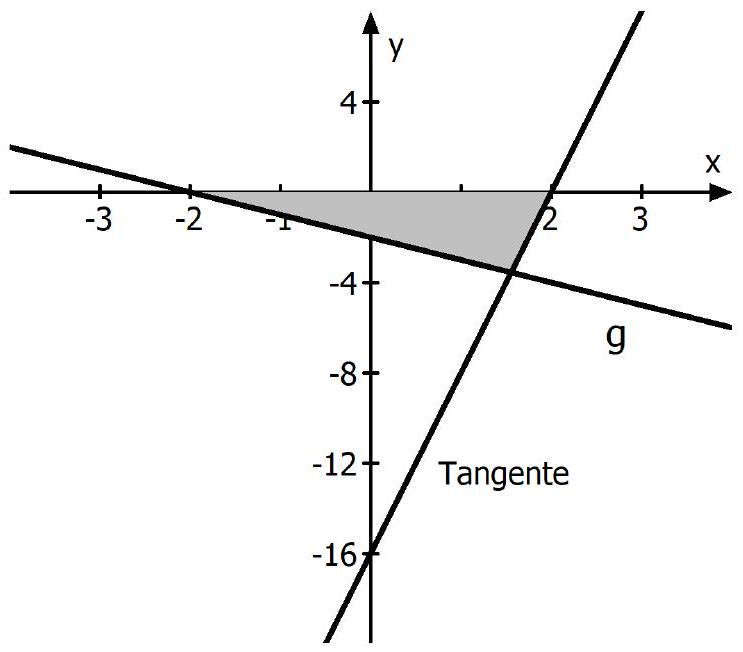
\includegraphics[max width=\textwidth, center]{2025_04_24_115a845b97d0fe4b6479g-5}

Schnittpunkt der Tangente und der Gerade g :\\
$8 x-16=-x-2 \Leftrightarrow 9 x=14 \Leftrightarrow x=\frac{14}{9}$\\
$y$-Wert des Schnittpunktes: $y=-\frac{14}{9}-2=-\frac{32}{9}$, also $S\left(\frac{14}{9} \left\lvert\,-\frac{32}{9}\right.\right)$\\
Dreiecksfläche: $\mathrm{A}=\frac{1}{2} \cdot 4 \cdot \frac{32}{9}=\frac{64}{9} \mathrm{FE}$\\
e) Beliebiger Punkt von dem Schaubild von f: $P(u \mid f(u))$

Mittelpunkt M der Strecke $\overline{\mathrm{OP}}: M\left(\frac{u+0}{2} \left\lvert\, \frac{f(u)+0}{2}\right.\right)$ also $M\left(\frac{u}{2} \left\lvert\, \frac{f(u)}{2}\right.\right)$\\
Nun soll gezeigt werden, dass der Punkt M auf dem Schaubild von h liegt:\\
Bedingung: $h\left(\frac{u}{2}\right)=\frac{f(u)}{2}$\\
$h\left(\frac{u}{2}\right)=4 \cdot\left(\frac{u}{2}\right)^{3}-4 \cdot \frac{u}{2}=4 \cdot \frac{u^{3}}{8}-2 u=\frac{1}{2} u^{3}-2 u$\\
Es gilt $\frac{f(u)}{2}=\frac{1}{2} \cdot f(u)=\frac{1}{2} \cdot\left(u^{3}-4 u\right)=\frac{1}{2} u^{3}-2 u$\\
Damit ist der Nachweis erbracht.

\section*{Aufgabe I 1.2}
a) Im Zeitraum 8:30 Uhr bis 10.00 Uhr sind $4364-1701=2663$ Lesebestätigungen eingegangen.\\
Dies entspricht einem Mittelwert von $\frac{2663}{1,5} \approx 1775$ Lesebestätigungen pro Stunde\\
b) Es gilt $k(2)=u(2)=1800$

Interpretation: Zum Zeitpunkt t = 2 (also um 9 Uhr) beträgt die momentane Änderungsrate der Anzahl der seit 7 Uhr eingegangenen Lesebestätigungen $1800 \frac{1}{\mathrm{~h}}$.\\
c) Das Schaubild der Funktion $v(x)=20 \cdot(x-18) \cdot(x-8)$ ist eine nach oben geöffnete Parabel mit den Nullstellen $x=8$ und $x=18$.\\
Das heißt für $8<x<18$ liegt die Parabel unterhalb der $x$-Achse.\\
Das würde bedeuten, dass sich in diesem Intervall negative Änderungsraten ergeben würden, was in diesem Sachzusammenhang jedoch nicht möglich ist.\\
d) Anzahl der Lesebestätigungen:

$$
\begin{aligned}
\int_{3}^{8} k(x) d x & =\int_{3}^{8}\left(20 x^{2}-520 x+2880\right) d x=\left[\frac{20}{3} x^{3}-260 x^{2}+2880 x\right]_{3}^{8} \\
& =9813, \overline{3}-6480 \approx 3333
\end{aligned}
$$

Im Zeitraum 10 Uhr bis 15 Uhr gehen ca. 3333 Lesebestätigungen ein.\\
Laut Tabelle gehen im Zeitraum 10 Uhr bis 15 Uhr 7572-4364 = 3208\\
Lesebestätigungen ein.\\
Prozentuale Abweichung: $\frac{3333-3208}{3208} \approx 0,039=3,9 \%$


\end{document}